\capitulo{6}{Trabajos relacionados}

En este apartado se van a observar distintas herramientas que como producto final generan mazmorras y con qué finalidad se utilizan.
Existen gran variedad de herramientas/juegos, tanto de pago como gratuitos en plataformas como itchio~\cite{itchio}, pero los siguientes engloban muy bien qué hay disponible.

\section{DunGen}
DunGen~\cite{DunGen} es una API web en la que se pueden generar mazmorras de alta resolución en dos dimensiones. Las mazmorras generadas se pueden descargar en formato .jpg de forma gratuita.

Este generador, ofrece incluir que sea multi-nivel, es decir, que tiene más de una planta además de que ofrece 8 temáticas para poder elegir, cambiando el aspecto de una mazmorra normal a una con temática de hielo. 
En esta herramienta, también se puede introducir si se desea la semilla al igual que en este proyecto.

Algo que no incluye es que poder introducir las dimensiones deseadas, en este caso da unas medidas por defecto y genera el resultado.
El resultado de una mazmorra generada tiene el aspecto de la figura 6.1.
\begin{figure}[ht!]  
    \centering  
    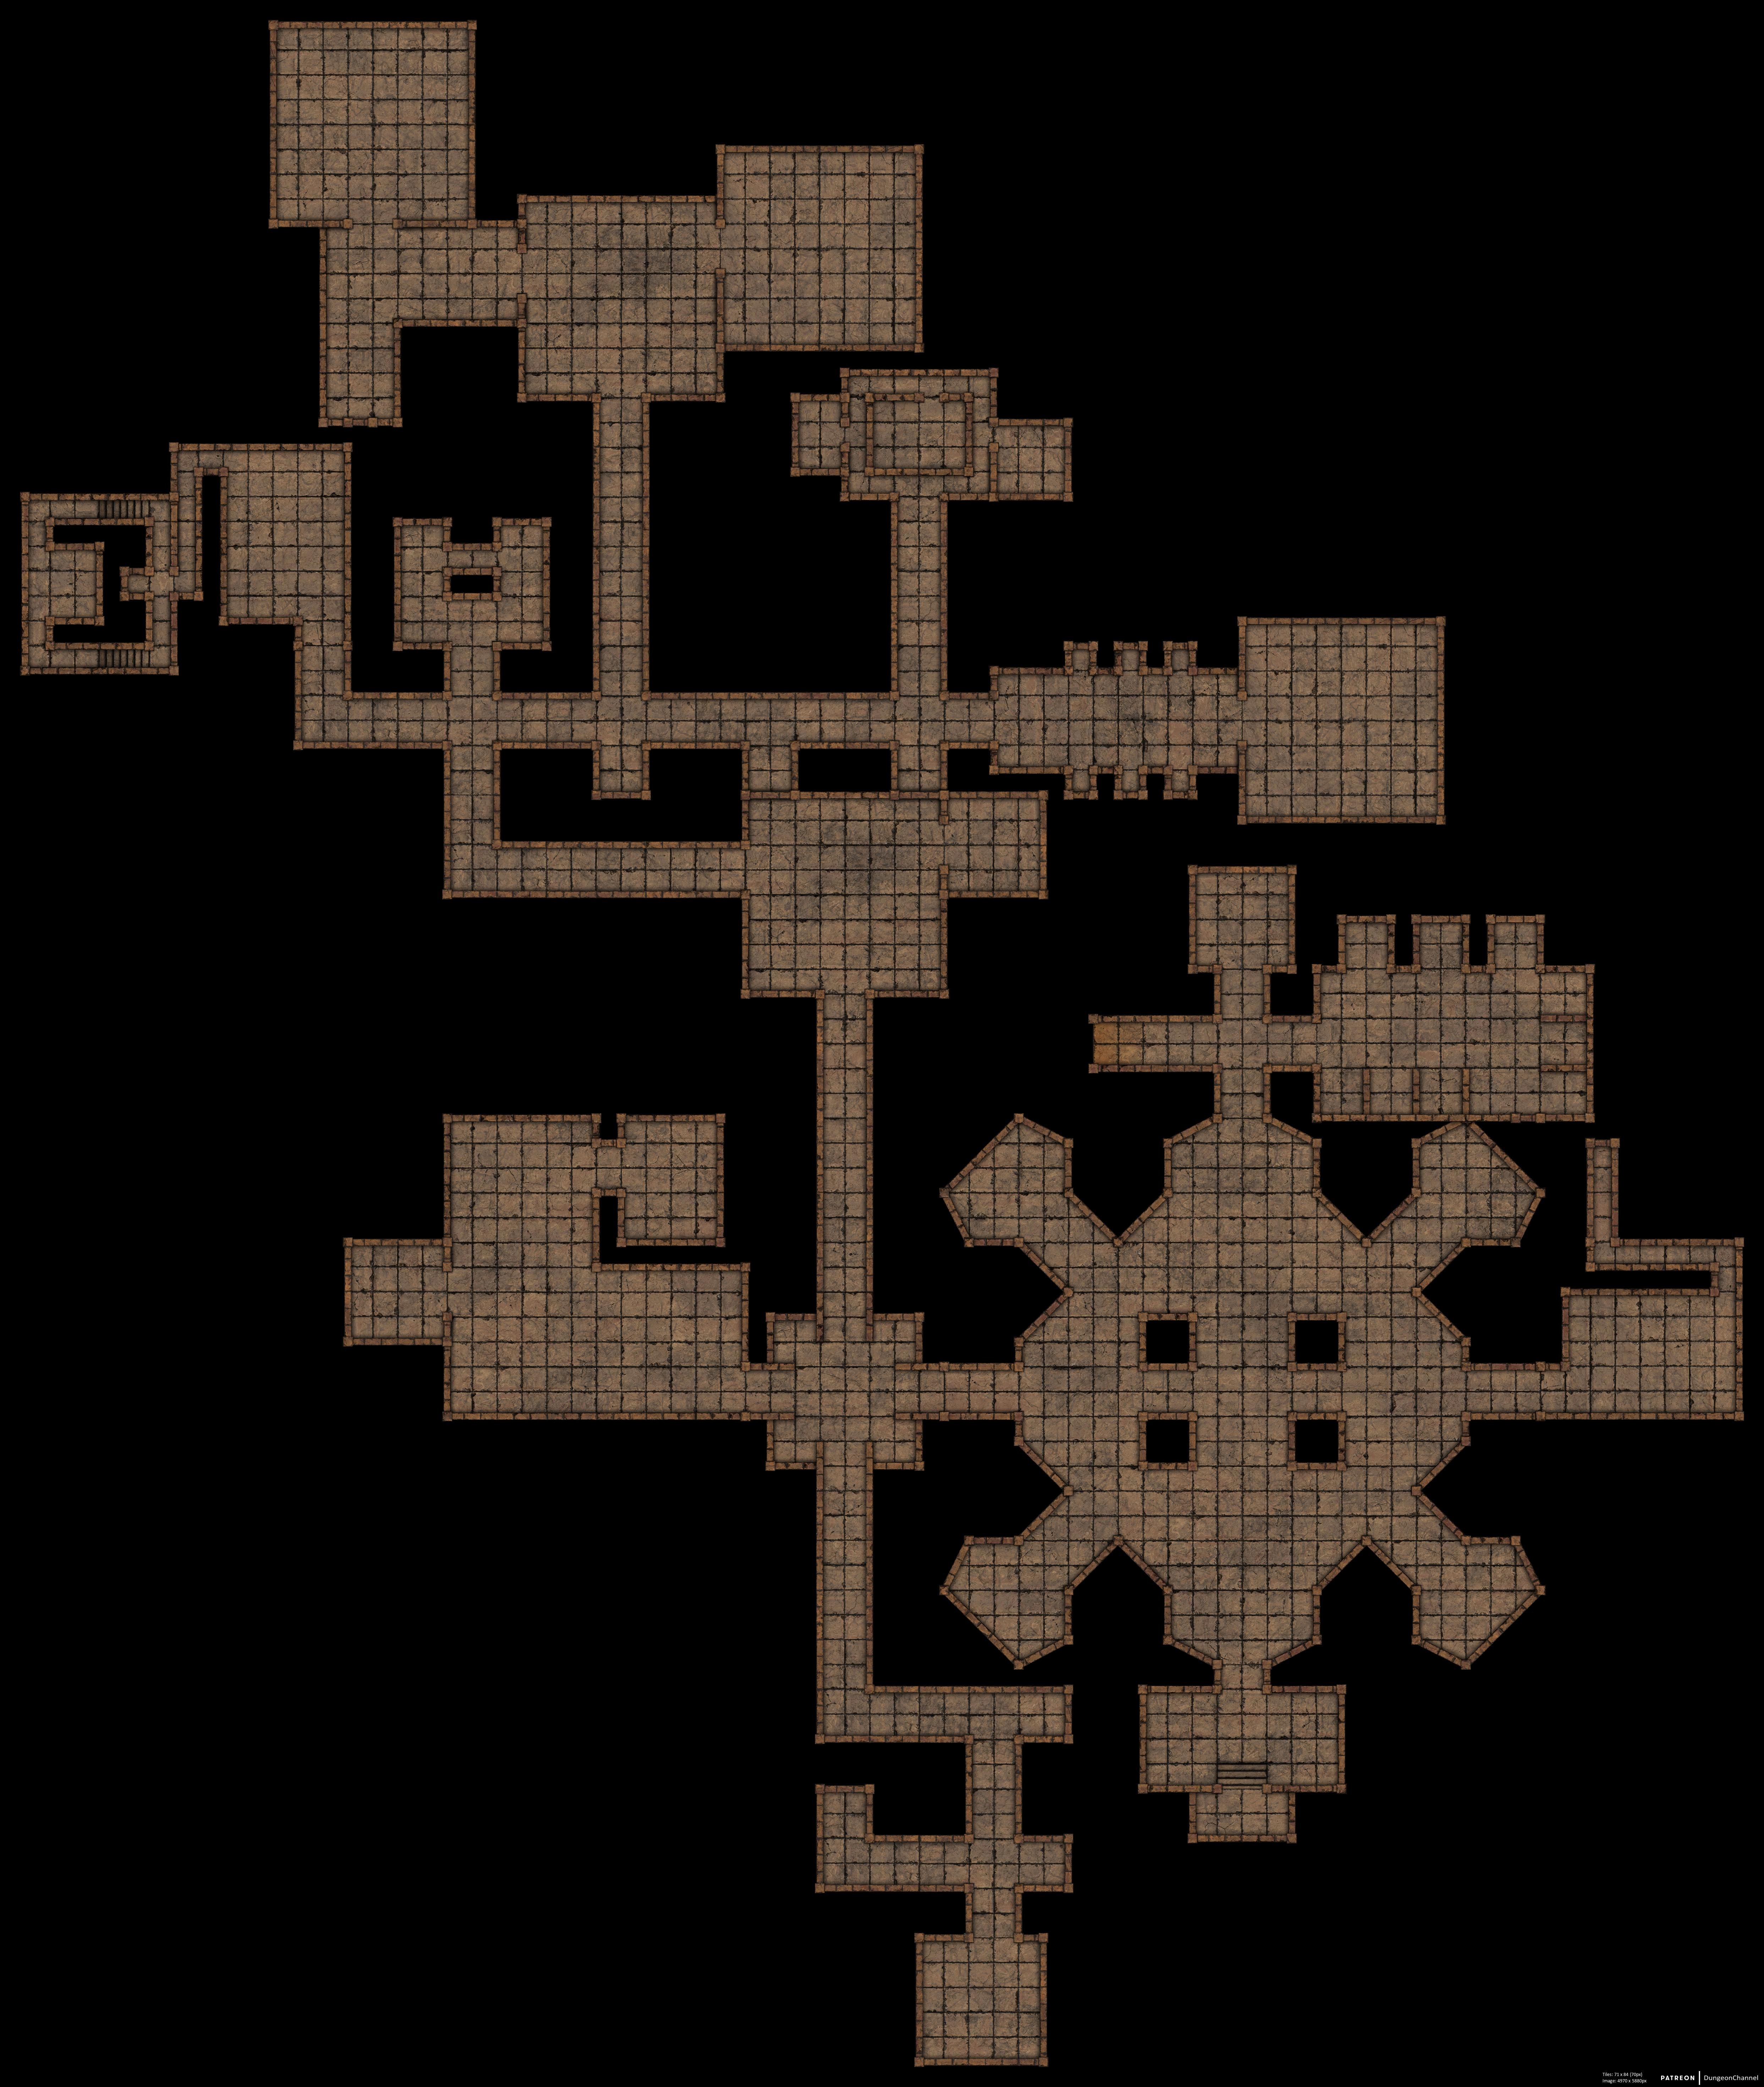
\includegraphics[width=\textwidth]{img/DunGenMediumExample.jpg}  
    \caption{Mazmorra generada con DunGen Dungeon Generator. Extraído de \url{https://dungen.app/dungen/}  }
    \label{fig:MazmorraDunGen}
\end{figure}

\section{Donjon}
Donjon~\cite{Donjon} es una API web que genera contenido para juegos de rol. Tiene un apartado para generar mazmorras, pero también genera gran cantidad de cosas como las puntuaciones de los enemigos o nombres de fantasía. Todo el contenido se puede descargar en varios formatos, haciendo de esta herramienta una muy versátil.
Este es un gran ejemplo de aplicación de generación de contenido fuera del ámbito de los videojuegos, funciona como herramienta de apoyo para crear un juego de mesa de rol propio.

La generación de mazmorras funciona de una forma similar a DunGen, mencionado anteriormente, pero a diferencia del anterior, este ofrece mucha más personalización, como por ejemplo, deja elegir si va a tener escaleras o si tiene puertas. Pero al igual que en el caso de DunGen, los parámetros ya están definidos, incluyendo el tamaño, es decir, no deja al usuario introducir manualmente el tamaño deseado.
Un ejemplo de resultado generado en Donjon tendría el aspecto de la figura \ref{fig:LabyrinthDonjon}.
\begin{figure}[h]  
    \centering  
    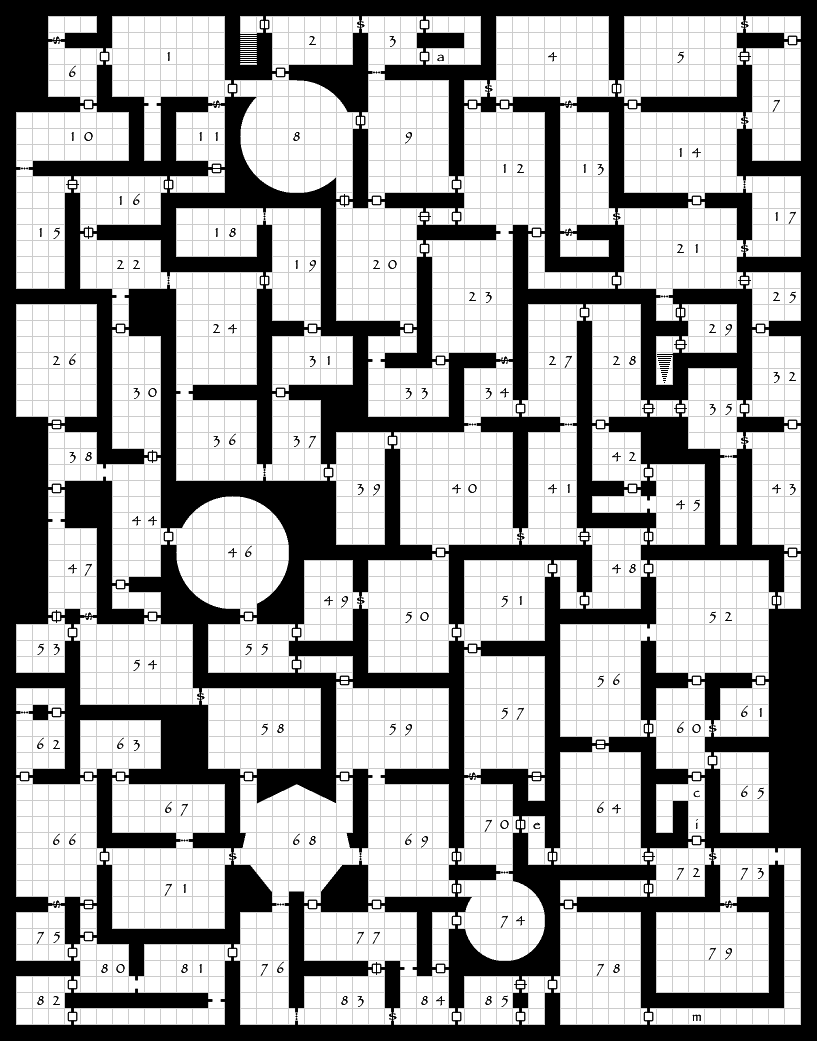
\includegraphics[width=\textwidth]{img/LabyrinthDonjon.png}  
    \caption{Mazmorra generada con Donjon.  Extraído de \url{https://donjon.bin.sh/d20/dungeon/}}  
    \label{fig:LabyrinthDonjon}
\end{figure}



\section{Endless RPG}

Endless RPG ~\cite{Endlessrpg}, es un juego de pago que genera mapas para Dragones y Mazmorras con enemigos y elementos clave para poder desarrollar la partida. El juego permite a los jugadores explorar la mazmorra y enfrentarse a los enemigos de la misma forma que se hace en una partida de rol, es decir, con un organizador de la partida que va gestionando los turnos y cómo los jugadores interactúan con el entorno. 

En este caso ya no es una herramienta para sólo generar mapas (o contenido), si no para poder jugar directamente, es muy completa y permite a los usuarios personalizar los mapas posicionando elementos para que los descubran los jugadores, como cofres y llaves para poder avanzar por las mazmorras.


\section{Maze Generator}
Más similar al resultado de este proyecto, Maze Generator~\cite{mazegenerator} es una herramienta que genera laberintos en 2D. Permite generar mazmorras de forma gratuita, se le pueden proporcionar datos como su ancho alto, desde dónde se comienza a recorrer el laberinto y el estilo de este. También permite exportar el laberinto generado a pdf o como imagen.
En este caso sí se pueden introducir las dimensiones deseadas pero no se tiene en cuenta la semilla. Tendría el aspecto como el de la figura \ref{fig:MazeGenerator}.
\begin{figure}[h]  
    \centering  
    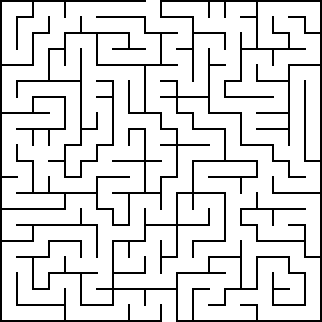
\includegraphics[width=\textwidth]{img/MazeGeneratorExample.png}  
    \caption{Laberinto generado con Maze Generator.}  
    \label{fig:MazeGenerator}
\end{figure}


